% LaTeX Template für Abgaben an der Universität Stuttgart
% Autor: Sandro Speth
% Bei Fragen: Sandro.Speth@iste.uni-stuttgart.de
%-----------------------------------------------------------
% Hauptmodul des Templates: Hier können andere Dateien eingebunden werden
% oder Inhalte direkt rein geschrieben werden.
% Kompiliere dieses Modul um eine PDF zu erzeugen.

% Dokumentenart. Ersetze 12pt, falls die Schriftgröße anzupassen ist.
\documentclass[12pt]{scrartcl}
% Einbinden der Pakete, des Headers und der Formatierung.
% Mit den \include und \input Befehlen können Dateien eingebunden werden:
% \include: Fügt einen Seitenumbruch nach dem Text ein
% \input: Fügt KEINEN Seitenumbruch nach dem Text ein
% LaTeX Template für Abgaben an der Universität Stuttgart
% Autor: Sandro Speth
% Bei Fragen: Sandro.Speth@iste.uni-stuttgart.de
%-----------------------------------------------------------
% Modul fuer verwendete Pakete.
% Neue Pakete einfach einfuegen mit dem \usepackage Befehl:
% \usepackage[options]{packagename}
\usepackage[utf8]{inputenc}
\usepackage[T1]{fontenc}
\usepackage[ngerman]{babel}
\usepackage{lmodern}
\usepackage{graphicx}
\usepackage[pdftex,hyperref,dvipsnames]{xcolor}
\usepackage{listings}
\usepackage[a4paper,lmargin={2cm},rmargin={2cm},tmargin={3.5cm},bmargin = {2.5cm},headheight = {4cm}]{geometry}
\usepackage{amsmath,amssymb,amstext,amsthm}
\usepackage[lined,algonl,boxed]{algorithm2e}
% alternative zu algorithm2e:
%\usepackage[]{algorithm} %counter mit chapter
%\usepackage{algpseudocode}
\usepackage{tikz}
\usepackage{hyperref}
\usepackage{url}
\usepackage[inline]{enumitem} % Ermöglicht ändern der enum Item Zahlen
\usepackage[headsepline]{scrlayer-scrpage} 
\pagestyle{scrheadings} 
\usetikzlibrary{automata,positioning}

% LaTeX Template für Abgaben an der Universität Stuttgart
% Autor: Sandro Speth
% Bei Fragen: Sandro.Speth@iste.uni-stuttgart.de
%-----------------------------------------------------------
% Modul beinhaltet Befehl fuer Aufgabennummerierung,
% sowie die Header Informationen.

% Überschreibt enumerate Befehl, sodass 1. Ebene Items mit
\renewcommand{\theenumi}{(\alph{enumi})}
% (a), (b), etc. nummeriert werden.
\renewcommand{\labelenumi}{\text{\theenumi}}

% Counter für das Blatt und die Aufgabennummer.
% Ersetze die Nummer des Übungsblattes und die Nummer der Aufgabe
% den Anforderungen entsprechend.
% Gesetz werden die counter in der hauptdatei, damit siese hier nicht jedes mal verändert werden muss
% Beachte:
% \setcounter{countername}{number}: Legt den Wert des Counters fest
% \stepcounter{countername}: Erhöht den Wert des Counters um 1.
\newcounter{sheetnr}
\newcounter{exnum}
\setcounter{sheetnr}{42}

% Befehl für die Aufgabentitel
\newcommand{\exercise}[1]{\section*{Aufgabe \theexnum\stepcounter{exnum}: #1}} % Befehl für Aufgabentitel

% Formatierung der Kopfzeile
% \ohead: Setzt rechten Teil der Kopfzeile mit
% Namen und Matrikelnummern aller Bearbeiter
\ohead{Jakob Rusch (3721483)}
% \chead{} kann mittleren Kopfzeilen Teil sezten
% \ihead: Setzt linken Teil der Kopfzeile mit
% Modulnamen, Semester und Übungsblattnummer
\ihead{Bachelor Ringvorlesung\\
Winter Term 2023/24\\
Übungsblatt \thesheetnr}

% Counter für das Blatt und die Aufgabennummer.
% Ersetze die Nummer des Übungsblattes und die Nummer der Aufgabe
% den Anforderungen entsprechend.
% Definiert werden die Counter in FormatAndHeader.tex
% Beachte:
% \setcounter{countername}{number}: Legt den Wert des Counters fest
% \stepcounter{countername}: Erhöht den Wert des Counters um 1.
\setcounter{sheetnr}{0} % Nummer des Übungsblattes
\setcounter{exnum}{1} % Nummer der Aufgabe

% Beginn des eigentlichen Dokuments
\begin{document}
% Nutze den \exercise{Aufgabenname} Befehl, um eine neue Aufgabe zu beginnen.
% Möchtest du eine Aufgabe in der Nummerierung überspringen, schreibe vor der Aufgabe: \stepcounter{exnum}
% Möchtest du die Nummer einer Aufgabe auf eine beliebige Zahl x setzen, schreibe vor der Aufgabe: \setcounter{exnum}{x}
\exercise{Table}
    \begin{table}[h]
        \centering
        \begin{tabular}{ c c c c }
            \hline
            \textbf{Name} & \textbf{Capital City} & \textbf{Population Density} & \textbf{Official Language(s)} \\
            \hline
            Germany & Berlin & 239 per \text{Km}{$^2$} & German \\
            The UK & London & 280 per \text{Km}{$^2$} & English \\
            The USA & Washington D.C. & 37 per \text{Km}{$^2$} & n/a \\
            China & Beijing & 152 per \text{Km}{$^2$} & Mandarin \\ 
            Japan & Tokyo & 338 per \text{Km}{$^2$} & Japanese \\
            \hline
        \end{tabular}
        \caption{Basic Statistics For Selected Countries}
        \label{fig:countries-statistics}
    \end{table}
\exercise{Funny Animal}
    \begin{figure}[t]
        \centering
        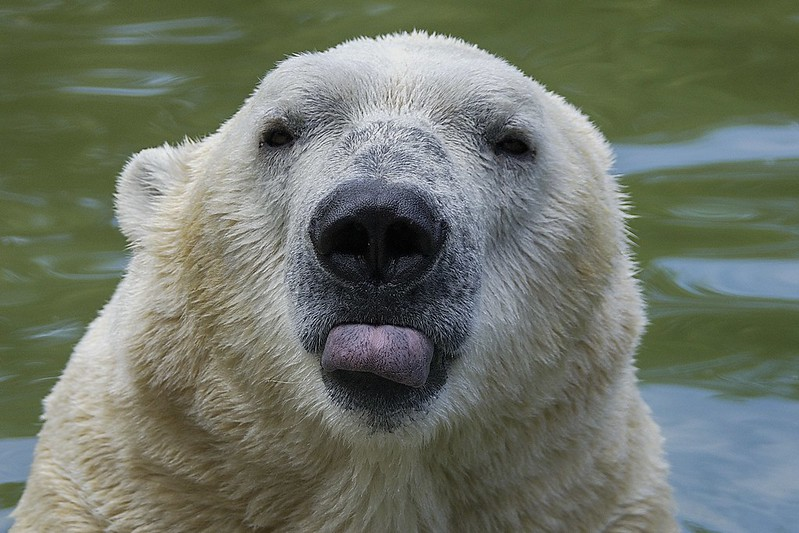
\includegraphics[width=0.8\linewidth]{images/funny_bear.jpg}
        \caption{A polar bear making a funny expression.}
        \label{fig:funny-animal-picture}
    \end{figure}
\exercise{Tikzpicture}
    \begin{figure}[h]
        \centering
        \begin{tikzpicture}[initial text={}]
            \node[state,initial] (A) {$A$};
            \node[state] (B) [below right=of A] {$B$};
            \node[state] (C) [right=of B] {$C$};
            \node[state,accepting] (D) [above right=of C] {$D$};
            \path[->] (A) edge node[above right]{$b$} (B);
            \path[->] (A) edge node[above]{$a$} (D);
            \path[->, loop left] (B) edge node{$b$} (B);
            \path[->] (B) edge node[above]{$a$} (C);
            \path[->, loop right] (C) edge node{$a$} (C);
            \path[->] (C) edge node[above left]{$b$} (D);
        \end{tikzpicture}        
        \caption{TikZ representation of Figure 1.}
        \label{fig:Figure_1}
    \end{figure}


\cite{s2011}

\bibliographystyle{plain}
\bibliography{literature}


% Ende des Dokuments
\end{document}
